\chapter{Pickup Project}
\label{pickup-project}

Some electric guitars uses pickups consisted by magnets wrapped on copper thin wire, they
\textit{work} \cite{pickup-work} using the variation of magnetic field, as the \textit{Faraday Law}
\cite{faraday-law}, created by the string vibration to generate the electrical signal correspondent
to each tone frequency.

\section{Requirements}
For assembly the pickup it was verified the requirements:

{\begin{itemize}
  \item pickup base to assembly the set up magnet+coil
  \item 6 magnets
  \item copper wire to wrap the magnets
  \item cover to attach the set up on the guitar
\end{itemize}}

\section{Pickup Base}
After some studies it was decided to print the pickup base using 3D printer, this
decision was due the reduction of the cost of the project. Than it was projected a 3D
model using the software AutoCAD and printed this on 3D printer as the project showed
on \autoref{3D-project}.

\begin{figure}[!htpb]
\centering
\caption{3D pickup base project}
\label{3D-project}
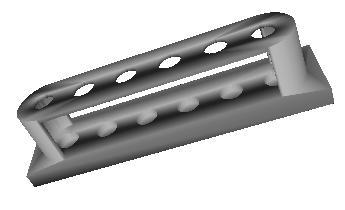
\includegraphics[scale=0.5]{images/pickup}
\legend{Source: made by authors}
\end{figure}

There was two materials to print the model, \textit{PLA} (Polylatic Acid) \cite{3d-materials}
and \textit{ABS} (Acrylonitrile Butadiene Styrene) \cite{3d-materials}. It was decided to print
the model on PLA because it attends the requisites of robustness of the project and it is
faster to print and have a lower cost when compared to the other material.

\section{Set up Magnets+Coils}

After print the pickup base it was assembled the coils around the guitar \autoref{magnets}
using thin copper wire. There was two dimensions of wire, 0.25mm and 0.5mm of diameter. It was
tested the set up with both wires and it was chosen to use on the project the 0.5mm
diameter wire because this dimension attended the pickup dimension restriction because it was
decided to give 500 turns on each magnet to reach a minimal desired voltage value of 1 V.

\begin{figure}[!htpb]
\centering
\caption{Magnets used on the project}
\label{magnets}
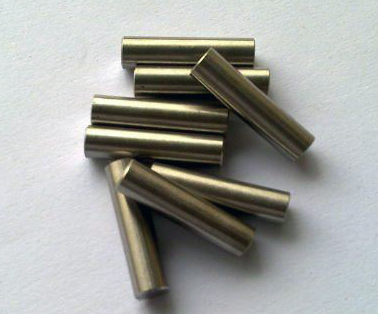
\includegraphics[scale=0.3]{images/magnets}
\legend{Source: \citeonline{pickup-magnets}}
\end{figure}

With the pickup already assembled it was verified the output signal. This signal
pick was less then 1 mV and this value was so weak to send to the Analog-digital
converter present on the microprocessor. With this dungeon it was verified that
it is requested a circuit responsible for the signal amplification to be possible to
read the signal with quality on the microprocessor.
